\chapter[MALHAS NÃO ESTRUTURADAS]{MALHAS NÃO ESTRUTURADAS}
\label{MALHAS NAO ESTRUTURADAS}
\section{Generalidades}

Uma malha não estruturada pode ser considerada um caso limite de uma malha multiblocos na qual cada volume individual é tratado como um bloco. A grande vantagem no uso de malhas não-estruturadas reside no fato de que não existe nenhuma estrutura (implícita) de linhas coordenadas que deva ser imposta à malha, o que permite que a malha seja facilmente concentrada (refinada) onde necessário, sem que haja desperdício de memória computacional. Além disso, os volumes de controle podem apresentar qualquer formato, não havendo restrições quanto ao número de volumes que compartilham um vértice (no caso 2D) ou uma linha (no caso 3D).

Usualmente, são empregados triângulos e quadriláteros no caso de problemas bidimensionais, e tetraedros e hexaedros em problemas tridimensionais. Outros formatos de volumes, no entanto, não são descartados.

O uso de malhas não-estruturadas esteve inicialmente relacionado ao método dos elementos finitos. Os trabalhos iniciais que empregam esse tipo de malha com volumes finitos são: \cite{winslow1966numerical}, \cite{baliga1980new}, \cite{baliga1983solution} e \cite{eiser1985trying}. Inicialmente, o método por eles empregado foi denominado de "métodos de elementos finitos baseados no volume de controle"(control volume based finite element methods - CVFEM). Segundo Maliska (2004), contudo, tal denominacão não é precisa, uma vez que balanços de propriedades são realizados sobre um volume de controle criado a partir de elementos (de malha); desta forma, a denominação mais adequada é a de "método de volumes finitos baseados em elementos" (element-based finite volume methods).

Quando se trabalha com malhas não-estruturadas, não ocorrem restrições quanto ao tipo de volume adotado (triângulos, quadriláteros, hexágonos, no caso 2D, tetraedros, hexaedros, no caso 3D). Em diversas situações, são empregados diferentes tipos de volume em diferentes regiões do domínio. Malhas não-estruturadas possuem como principal atrativo o fato de que permitem a discretização de domínios arbitrários, com elevada complexidade. Pode-se, também, realizar refinamentos locais de malhas, em regiões que apresentam elevado gradiente de propriedades.

Existem duas formas de definir volumes de controle em malhas não-estruturadas:
\begin{itemize}
    \item volumes de controle centrados nos elementos;
    \item volumes de controle baseados nos vértices. Ambas as formas são encontradas na literatura.
\end{itemize}

No caso de volumes de controle centrados nos elementos, os nós são dispostos nos centroides dos volumes de controle. O centroide ou centro de gravidade de um volume, é definido como:

\begin{equation}
    \label{eq:6.1}
    x_c = \frac{\int_{vc}x dv}{\int_{vc}dv};
    y_c = \frac{\int_{vc}y dv}{\int_{vc}dv};
    z_c = \frac{\int_{vc}z dv}{\int_{vc}dv}
\end{equation}

No caso bidimensional, tem-se:

\begin{equation}
    \label{eq:6.2}
    x_c = \frac{\int_{vc}x dv}{\int_{vc}dv};
    y_c = \frac{\int_{vc}y dv}{\int_{vc}dv};
\end{equation}

No caso de triângulos, pode-se provar que:

\begin{equation}
    \label{eq:6.3}
    x_c = \frac{x_1+x_2+x_3}{3};
    y_c = \frac{y_1+y_2+y_3}{3}
\end{equation}

e

\begin{equation*}
    2A = det \begin{vmatrix}
        x_1 & y_1 & 1\\
        x_2 & y_2 & 1\\
        x_3 & y_3 & 1
    \end{vmatrix}
    = x_1y_2 + x_2y_3 + x_3y_1 - x_3y_2 - x_2y_1 - x_1y_3
\end{equation*}

ou seja,

\begin{equation}
    \label{eq:6.4}
    A = \frac{1}{2}(x_1y_2 + x_2y_3 + x_3y_1 - x_3y_2 - x_2y_1 - x_1y_3)
\end{equation}

Quando se emprega a metodologia de volumes de controle baseados nos vértices, os nós são dispostos nos vértices dos elementos de malha, neste caso, torna-se necessário construir os volumes ao redor dos centroides. Neste caso, o método mais empregado é o chamado método das medianas. Deve-se conectar os pontos médios dos segmentos de reta que formam os lados dos polígonos, no caso 2D, ou que formam as arestas dos poliedros, no caso 3D, aos centroides dos polígonos/poliedros correspondentes. Gera-se, assim, um volume de controle em cujo interior se encontra o vértice do polígono/poliedro.

Será abordado o método de volumes de controle centrados nos elementos, uma vez que sua compreensão é mais simples e seus requerimentos de memória são menores, uma vez que em uma malha sempre ocorrem mais vértices que centroides.

A discretização em malhas não-estruturadas pode ser realizada partindo-se da técnica básica de volumes de controle, na qual é empregada a forma integral das equações de conservação como ponto de partida:

\begin{equation}
    \label{eq:6.5}
    \int_{vc} \frac{\partial}{\partial t} (\rho \phi) dv + \int_{vc} \vec{\Delta} \cdot (\rho \phi \vec{u}) dv = \int_{vc} \vec{\Delta} \cdot (\Gamma \vec{\Delta} \phi) dv + \int_{vc} S^\phi dv
\end{equation}

As integrais volumétricas do termo transiente e do termo fonte podem ser convenientemente estimados como o produto entre o volume do elemento de malha e o valor apresentado no centroide do volume (no integrando).

A equação \ref{eq:6.5} apresenta, ainda, termos advectivos $(\rho \phi \vec{u})$ e difusivos $(\Gamma \vec{\Delta} \phi)$. Quando da ausência de um sistema específico de coordenadas, é necessário um cuidadoso tratamento desses termos. Recordando-se do teorema da divergência de Gauss, aplicável a qualquer tipo de volume de controle:

\begin{equation}
    \label{eq:6.6}
    \int_{vc}\vec{\Delta} \cdot \vec{a} dv = \int_A \hat{n} \cdot \hat{a} dA
\end{equation}

A integral de superfície deve ser realizada sobre a fronteira A do volume de controle vc. A interpretação física de $\hat{n} \cdot \hat{a}$ reside na componente do vetor $\vec{a}$ na direção do vetor normal $\hat{n}$ (externo à superfície) para um elemento superficial infinitesimal $dA$.

A aplicação do teorema da divergência de Gauss na equação \ref{eq:6.5} origina:

\begin{equation}
    \label{eq:6.7}
    \frac{\partial}{\partial t}\int_{vc} (\rho \phi dv) + \int_A \hat{n} \cdot (\rho \phi \vec{u}) dA = \int_A \hat{n} \cdot (\Gamma \vec{\Delta} \phi)dA + \int_{vc}S^\phi dv
\end{equation}

Nota-se qua A indica a superfície total que envolve o volume de controle vc, enquanto $dA$ é um elemento infinitesimal de superfície. As integrais de superfície podem ser avaliadas sobre todos os segmentos de reta (2D) ou elementos de área (3D) de modo que a equação \ref{eq:6.7} pode ser expressa como:

\begin{equation}
    \label{eq:6.8}
    \frac{\partial}{\partial t}(\int_{vc}\rho \phi dv) + \sum_{\text{superfícies}} \int_{\Delta A_i} \hat{n_i} (\rho \phi \vec{u}) dA= \sum_{\text{superfícies}} \int_{\Delta A_i} \hat{n_i} \cdot (\Gamma \vec{\Delta} \phi) dA + \int_{vc} S^\phi dv
\end{equation}

No caso de regime permanente, tem-se:

\begin{equation}
    \label{eq:6.9}
    \int_A \hat{n} \cdot (\phi \phi \vec{u}) dA = \int_A \hat{n} \cdot (\Gamma \vec{\Delta} \phi) dA + \int_{vc} S^\phi dv
\end{equation}

e então,

\begin{equation}
    \label{eq:6.10}
    \sum_{\text{superfícies}} \int_{\Delta A_i} \hat{n_i} \cdot (\rho \phi \vec{u}) dA = \sum_{\text{superfícies}} \int_{\Delta A_i} \hat{n_i} \cdot (\Gamma \vec{\Delta} \phi) dA + \int_{vc} S^\phi dv
\end{equation}

Para calcular-se as integrais de superfície, são necessárias expressões para os vetores de fluxo $(\rho \phi \vec{u})$ e $(\Gamma \vec{\Delta} \phi)$, assim como para as quantidades geométricas $\hat{n_i}$ e $\Delta A_i$ conforme a figura \ref{fig:geometrias}.

\begin{figure}[h]
    \centering
    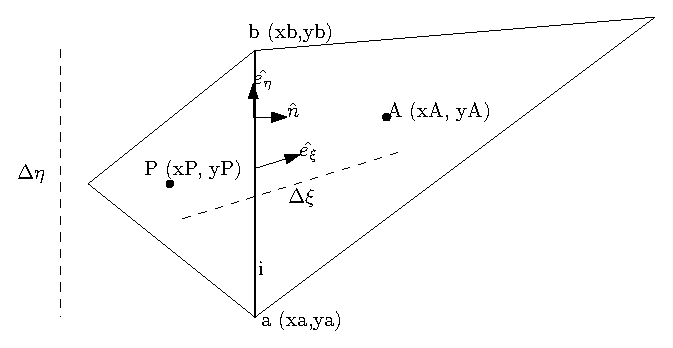
\includegraphics{fig/geometrias.eps}
    \caption{Geometrias para cálculos das expressões}
    \label{fig:geometrias}
\end{figure}

Na figura \ref{fig:geometrias}, P é o centroide do volume de controle para o qual a discretização é feita. O ponto A corresponde ao centroide do volume de controle vizinho e $\hat{e_\xi}$ é um vetor unitário (versor) na direção da linha que une os pontos P e A. A face i separa os dois volumes de controle e a-b é uma linha que une os pontos a e b, vértices compartilhados por ambos os volumes. As coordenadas dos pontos a e b são $(x_a, y_a)$ e $(x_b, y_b)$, respectivamente, enquanto $\hat{n}$ e $\hat{e_\eta}$ são, respectivamente, o vetor unitário normal (direcionado para fora do volume) e o vetor unitário tangente à face i.

Considerando-se a face i, apresentada na figura \ref{face-i} temos:

\begin{figure}[h]
    \centering
    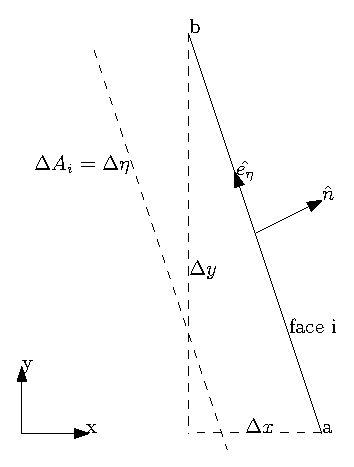
\includegraphics{fig/face-i.eps}
    \caption{Face i}
    \label{face-i}
\end{figure}

Tem-se que a área de tal face é calculada como:

\begin{equation}
    \label{eq:6.11}
    \Delta A_i = \sqrt{(\Delta x)^2 + (\Delta y)^2}
\end{equation}

Sendo:

\begin{equation}
    \label{eq:6.12}
    \Delta x = x_b - x_a
\end{equation}

\begin{equation}
    \label{eq:6.13}
    \Delta y = y_b - y_a
\end{equation}

O vetor unitário normal à superfície i é definida como:

\begin{equation}
    \label{eq:6.14}
    \hat{n} = \frac{\Delta y}{\Delta A_i}\hat{i} - \frac{\Delta x}{\Delta A_i}\hat{j}
\end{equation}

Na ausência de uma estrutura de malha, é necessário criar uma estrutura de dados para as informações geométricas, identificando a relação entre vértices, índices dos volumes, faces relevantes e volumes vizinhos (conectividades).

\section{Geração de malhas triangulares}

Malhas com elementos triangulares (ou tetraédricos) são malhas versáteis que podem preencher com facilidade domínios bastante irregulares, mas apresentam a dificuldade de ordenação que implica em matrizes de coeficientes sem a estrutura de bandas.

Como qualquer tipo de malha, malhas triangulares devem obedecer a certos requisitos, ou possuir certas propriedades, para que a solução numérica tenha qualidade. As propriedades de uma malha são definidas pelo número, forma e tamanho dos elementos, sendo o tempo de CPU e a memória utilizados para a geração também parâmetros importantes. Satisfazer os critérios de boa qualidade de malha e minimizar o tempo de processamento são processos contrários, pois melhorar a qualidade de uma malha significa, quase sempre, em aumentar o esforço computacional. Dessa contradição vem a dificuldade de criar-se geradores versáteis e rápidos e qu atendam aos requisitos numéricos.

Depois de bem representada através das superfícies, a fronteira de cálculo deve coincidir o melhor possível com a malha. Deste modo, tem-se que uma das mais importantes propriedades da malha é a sua coincidência com a fronteira, uma vez que disso depende a correta aplicação das condições de contorno. O controle do tamanho dos elementos é um parâmetro que é facilmente incluído em um gerador de malhas, o controle da forma dos elementos, contudo, é algo mais difícil de se conseguir.

Para uma malha que utilize elementos triangulares, é desejável que os mesmos sejam o mais próximo possível de triângulos equiláteros, pois isto permite que as funções de interpolação representem bem as variáveis dentro do triângulo. Quando um triângulo se afasta por demais do padrão equilátero, tem-se o equivalente a um elemento com elevada razão de aspecto em malhas com quadriláteros. Neste caso, observa-se uma elevada anisotropia nos coeficientes, o que reduz a taxa de convergência do processo de solução do sistema linear.

Além disso, é necessário que as dimensões do elemento variem de forma suave dentro do domínio e não de forma brusca, de modo a evitar volumes de controle irregulares, no qual o centroide se localiza próximo a duas faces do volume e, portante, não se configura em um ponto representativo de todo o volume de controle. É importante, assim, que a malha apresente certa uniformidade.

Outra propriedade de um gerador deve ser sua capacidade de adequação ao problema físico. Isto deve ser feito externamente ao gerador, pois é necessário que se conheça o comportamento da solução, de modo a se gerar a malha com refinamento em locais onde seja requerido. A forma automática de se executar essa tarefa, denominada adaptabilidade, é um ponto forte do gerador.

\begin{figure}[ht]
    \begin{subfigure}{.5\textwidth}
        \centering
        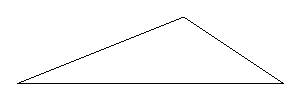
\includegraphics[width=.8\linewidth]{fig/escaleno.eps}
        \caption{Elemento escaleno}
        \label{fig:sub-escaleno}
    \end{subfigure}
    \begin{subfigure}{.5\textwidth}
        \centering
        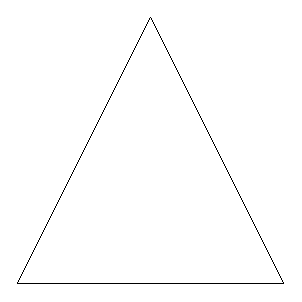
\includegraphics[width=.4\linewidth]{fig/equilatero.eps}
        \caption{Elemento equilátero}
        \label{fig:sub-second}
    \end{subfigure}

    \begin{subfigure}{.5\textwidth}
        \centering
        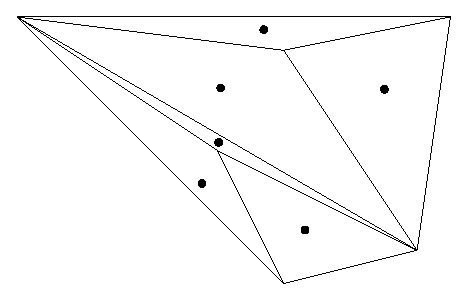
\includegraphics[width=.8\linewidth]{fig/variacao_brusca.eps}
        \caption{Variação brusca nas dimensões dos elementos}
        \label{fig:sub-brusca}
    \end{subfigure}
    \begin{subfigure}{.5\textwidth}
        \centering
        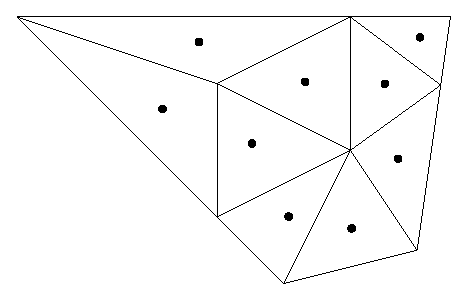
\includegraphics[width=.8\linewidth]{fig/variacao_suave.eps}
        \caption{Malha com variação mais suave dos elementos}
        \label{fig:sub-suave}
    \end{subfigure}
    \caption{Comparação de elementos desejáveis/indesejáveis}
    \label{fig:figlegal}
\end{figure}
